%%%%%%%%%%%%%%%%%%%%%%%%%%%%%%%%%%%%%%%%%%%%%%%%%%%%%%%%%%%%%%%%%%%%% 
%% This is a (brief) model paper using the achemso class 
%% The document class accepts keyval options, which should include 
%% the target journal and optionally the manuscript type. 
%%%%%%%%%%%%%%%%%%%%%%%%%%%%%%%%%%%%%%%%%%%%%%%%%%%%%%%%%%%%%%%%%%%%% 
\documentclass[journal=jctcce,manuscript=article]{achemso} 
 
%%%%%%%%%%%%%%%%%%%%%%%%%%%%%%%%%%%%%%%%%%%%%%%%%%%%%%%%%%%%%%%%%%%%% 
%% Place any additional packages needed here.  Only include packages 
%% which are essential, to avoid problems later. Do NOT use any 
%% packages which require e-TeX (for example etoolbox): the e-TeX 
%% extensions are not currently available on the ACS conversion 
%% servers. 
%%%%%%%%%%%%%%%%%%%%%%%%%%%%%%%%%%%%%%%%%%%%%%%%%%%%%%%%%%%%%%%%%%%%% 

%% Workaround for malfunctioning textsuperscript with pdfx and T1 encoding
\let\tmpa\textsuperscript
\DeclareTextCommandDefault{\textsuperscript}{\tmpa}

\usepackage[x11names]{xcolor}  % typesetting in color
%% Generate PDF/A-2u
%\usepackage[a-2u]{pdfx}
 
\usepackage[super]{natbib}         % citation style AUTHOR (YEAR), or AUTHOR [NUMBER]

\usepackage{achemso}  
\usepackage{rotating}  
%\usepackage{times} 
%\usepackage{lmodern}    %% Prefer Latin Modern fonts
\usepackage{graphicx} 
\usepackage{setspace} 
\usepackage{amsmath} 
\usepackage{epstopdf} 
\usepackage{csquotes} 
\usepackage{mhchem} 
\usepackage{chemfig} 
\usepackage[obeyFinal]{easy-todo}
\usepackage[english]{babel}
\usepackage{xr}
\externaldocument{manuscriptSUPPL}


\usepackage{subfig}
\usepackage{dcolumn}        % improved alignment of table columns
\usepackage{booktabs}       % improved horizontal lines in tables
\usepackage{paralist}       % improved enumerate and itemize

%% Character encoding: usually latin2, cp1250 or utf8:
\usepackage[utf8]{inputenc}
\usepackage[T1]{fontenc}

%\usepackage{markdown}  
 
%% The hyperref package for clickable links in PDF and also for storing
%% metadata to PDF (including the table of contents).
%% Most settings are pre-set by the pdfx package.
%\hypersetup{unicode}
%\hypersetup{breaklinks=true}
%\hypersetup{colorlinks,allcolors=DodgerBlue4}
 
%%%%%%%%%%%%%%%%%%%%%%%%%%%%%%%%%%%%%%%%%%%%%%%%%%%%%%%%%%%%%%%%%%%%% 
%% If issues arise when submitting your manuscript, you may want to 
%% un-comment the next line.  This provides information on the 
%% version of every file you have used. 
%%%%%%%%%%%%%%%%%%%%%%%%%%%%%%%%%%%%%%%%%%%%%%%%%%%%%%%%%%%%%%%%%%%%% 
%%\listfiles 
 
%%%%%%%%%%%%%%%%%%%%%%%%%%%%%%%%%%%%%%%%%%%%%%%%%%%%%%%%%%%%%%%%%%%%% 
%% Place any additional macros here.  Please use \newcommand* where 
%% possible, and avoid layout-changing macros (which are not used 
%% when typesetting). 
%%%%%%%%%%%%%%%%%%%%%%%%%%%%%%%%%%%%%%%%%%%%%%%%%%%%%%%%%%%%%%%%%%%%% 
\newcommand*\mycommand[1]{\texttt{\emph{#1}}} 
%%% Custom variables
% width suitable for fitting into a column in 1-column page layout
\newlength{\figwidth}
\setlength{\figwidth}{9 cm} 
\newlength{\figwidthsmall}
\setlength{\figwidthsmall}{6 cm} 
\newlength{\figwidthfull}
\setlength{\figwidthfull}{16 cm} 
\newlength{\figheightsmall}
\setlength{\figheightsmall}{6 cm} 
\newlength{\figheight}
\setlength{\figheight}{12 cm} 

 
%%%%%%%%%%%%%%%%%%%%%%%%%%%%%%%%%%%%%%%%%%%%%%%%%%%%%%%%%%%%%%%%%%%%% 
%% Meta-data block 
%% --------------- 
%% Each author should be given as a separate \author command. 
%% 
%% Corresponding authors should have an e-mail given after the author 
%% name as an \email command. Phone and fax numbers can be given 
%% using \phone and \fax, respectively; this information is optional. 
%% 
%% The affiliation of authors is given after the authors; each 
%% \affiliation command applies to all preceding authors not already 
%% assigned an affiliation. 
%% 
%% The affiliation takes an option argument for the short name.  This 
%% will typically be something like "University of Somewhere". 
%% 
%% The \altaffiliation macro should be used for new address, etc. 
%% On the other hand, \alsoaffiliation is used on a per author basis 
%% when authors are associated with multiple institutions. 
%%%%%%%%%%%%%%%%%%%%%%%%%%%%%%%%%%%%%%%%%%%%%%%%%%%%%%%%%%%%%%%%%%%%% 
 
\author{Josef Melcr} 
\email{melcr@marge.uochb.cas.cz} 
%%\homepage[]{https://jmelcr.github.io/}
\affiliation{Institute of Organic Chemistry and Biochemistry, 
Czech Academy of Sciences,  
Prague 6, Czech Republic} 
\author{Tiago Ferreira}
\affiliation{NMR group - Institut for Physics, Martin-Luther University Halle-Wittenberg} 
\author{Pavel Jungwirth} 
%%\homepage[]{http://jungwirth.uochb.cas.cz/}
\affiliation{Institute of Organic Chemistry and Biochemistry, 
Czech Academy of Sciences,  
Prague 6, Czech Republic} 
\author{O. H. Samuli Ollila} 
\email{samuli.ollila@helsinki.fi} 
%%\homepage[]{Your web page} 
\affiliation{Institute of Organic Chemistry and Biochemistry, 
Czech Academy of Sciences,  
Prague 6, Czech Republic} 
\alsoaffiliation{Institute of Biotechnology, University of Helsinki} 
 
 
%%%%%%%%%%%%%%%%%%%%%%%%%%%%%%%%%%%%%%%%%%%%%%%%%%%%%%%%%%%%%%%%%%%%% 
%% The document title should be given as usual. Some journals require 
%% a running title from the author: this should be supplied as an 
%% optional argument to \title. 
%%%%%%%%%%%%%%%%%%%%%%%%%%%%%%%%%%%%%%%%%%%%%%%%%%%%%%%%%%%%%%%%%%%%% 
%\title[] 
%  {Accurate interactions of cations with 
%   neutral and negatively charged membranes 
%   via combination of experiments and molecular simulation}

\title[] 
      {Improved Cation Binding to Lipid Bilayer with
Negatively Charged POPS by Effective
Inclusion of Electronic Polarization}

%%%%%%%%%%%%%%%%%%%%%%%%%%%%%%%%%%%%%%%%%%%%%%%%%%%%%%%%%%%%%%%%%%%%% 
%% Some journals require a list of abbreviations or keywords to be 
%% supplied. These should be set up here, and will be printed after 
%% the title and author information, if needed. 
%%%%%%%%%%%%%%%%%%%%%%%%%%%%%%%%%%%%%%%%%%%%%%%%%%%%%%%%%%%%%%%%%%%%% 
\abbreviations{IR,NMR,UV,MD,ECC,PC,PS,POPS,POPS} 
\keywords{MD simulation, molecular modeling, 
          polarizability, polarization,
          phospholipids, phosphatidylserine} 

%%%%%%%%%%%%%%%%%%%%%%%%%%%%%%%%%%%%%%%%%%%%%%%%%%%%%%%%%%%%%%%%%%%%% 
%% The manuscript does not need to include \maketitle, which is 
%% executed automatically. 
%%%%%%%%%%%%%%%%%%%%%%%%%%%%%%%%%%%%%%%%%%%%%%%%%%%%%%%%%%%%%%%%%%%%% 
\begin{document} 
 
%%%%%%%%%%%%%%%%%%%%%%%%%%%%%%%%%%%%%%%%%%%%%%%%%%%%%%%%%%%%%%%%%%%%% 
%% The "tocentry" environment can be used to create an entry for the 
%% graphical table of contents. It is given here as some journals 
%% require that it is printed as part of the abstract page. It will 
%% be automatically moved as appropriate. 
%%%%%%%%%%%%%%%%%%%%%%%%%%%%%%%%%%%%%%%%%%%%%%%%%%%%%%%%%%%%%%%%%%%%% 
\begin{tocentry} 
 
Some journals require a graphical entry for the Table of Contents. 
This should be laid out ``print ready'' so that the sizing of the 
text is correct. 
 
Inside the \texttt{tocentry} environment, the font used is Helvetica 
8\,pt, as required by \emph{Journal of the American Chemical 
Society}. 
 
The surrounding frame is 9\,cm by 3.5\,cm, which is the maximum 
permitted for  \emph{Journal of the American Chemical Society} 
graphical table of content entries. The box will not resize if the 
content is too big: instead it will overflow the edge of the box. 
 
This box and the associated title will always be printed on a 
separate page at the end of the document. 
 
\end{tocentry} 
 
%%%%%%%%%%%%%%%%%%%%%%%%%%%%%%%%%%%%%%%%%%%%%%%%%%%%%%%%%%%%%%%%%%%%% 
%% The abstract environment will automatically gobble the contents 
%% if an abstract is not used by the target journal. 
%%%%%%%%%%%%%%%%%%%%%%%%%%%%%%%%%%%%%%%%%%%%%%%%%%%%%%%%%%%%%%%%%%%%% 
 
 
 
\begin{abstract} 
  Phosphatidylserine (PS) lipids are important signaling molecules and the most common negatively charged lipids in eukaryotic membranes.
  The signaling can be often regulated by calcium, but its interactions with PS headgroups are not fully understood.
  Classical molecular dynamics (MD) simulations can potentially give detailed description of lipid-ion interactions,
  but the results strongly depend on the used force field. Here, we apply the electronic continuum correction (ECC) to
  the Amber Lipid17 parameters of 1-palmitoyl-2-oleoyl-{\it sn}-glycero-3-phospho-L-serine (POPS) lipid to improve its
  interactions with Na$^+$ and Ca$^{2+}$ ions.
  The partial charges of headgroup, glycerol backbone and carbonyls of POPS, bearing a unit negative charge, were scaled with a
  factor of 0.75, derived for monovalent ions and the Lennard-Jones $\sigma$ parameters of the same segments were scaled with a factor of 0.89.
  The resulting ECC-POPS model gives more realistic interactions with Na$^+$ and Ca$^{2+}$ cations than the original Amber Lipid17 parameters,
  when validated using headgroup order parameters and ''electrometer concept''.
  In ECC-lipids simulations, Ca$^{2+}$ cations do not simultaneously interact with more than two PS lipids, and interactions 
  with carboxylate groups is twice more likely than with phosphate groups, while interaction with carbonyls is almost negligible.
  Our results pave the way for more realistic MD simulations of anionic biological membranes and demonstrate the 
  usefulness of ECC also to charged lipids.
\end{abstract} 
 
 
%\begin{abstract} 
%  This is an example document for the \textsf{achemso} document 
%  class, intended for submissions to the American Chemical Society 
%  for publication. The class is based on the standard \LaTeXe\ 
%  \textsf{report} file, and does not seek to reproduce the appearance 
%  of a published paper. 
 
%  This is an abstract for the \textsf{achemso} document class 
%  demonstration document.  An abstract is only allowed for certain 
%  manuscript types.  The selection of \texttt{journal} and 
%  \texttt{manuscript} will determine if an abstract is valid.  If 
%  not, the class will issue an appropriate error. 
%\end{abstract} 
 
%%%%%%%%%%%%%%%%%%%%%%%%%%%%%%%%%%%%%%%%%%%%%%%%%%%%%%%%%%%%%%%%%%%%% 
%% Start the main part of the manuscript here. 
%%%%%%%%%%%%%%%%%%%%%%%%%%%%%%%%%%%%%%%%%%%%%%%%%%%%%%%%%%%%%%%%%%%%% 
 
 
 
\section{Introduction} 

Phosphatidylserine (PS) lipids are the most common negatively charged lipids in eukaryotic membranes
and important signaling molecules \cite{lemmon08,leventis10,li14}.
They interact with signaling proteins \cite{leventis10},
regulate surface charge and protein localization \cite{yeung08}, 
induce protein aggregation \cite{zhao04,gorbenko06} and membrane fusion \cite{wilschut1981calcium, papahadjopoulos90, verma2018cell}.
As such lipid-related functions are also often regulated by ions \cite{leventis10},
a detailed understanding of interactions between negatively charged lipids and biologically relevant cations such as calcium is of a great importance.
Recent combination of spectroscopic experiments, biochemical essays, and molecular simulations showed that binding of
calcium to \ce{PIP_2} lipids inhibits their recognition by a phospolipase~C, 
which demonstrates that not only proteins but also lipids can get involved in calcium signaling \cite{Bilkova2017Calcium}.

Spectroscopic experiments give accurate information about the
interactions between ions and PS lipids, but the data is often indirect and difficult to
interpret \cite{hauser77,kurland79,eisenberg79,hauser83,dluhy83,hauser85,feigenson86,mattai89,roux90,roux91}.
Some studies suggest that the
binding affinity of ions to negatively charged lipids is similar to that of zwitterionic lipids,
and the binding affinity is increased only due to the increased cation
concentration in the vicinity of the membrane \cite{seelig90,sinn06}.
On the other hand, calcium forms dehydrated complexes with PS headgroups
which cause phase separation \cite{hauser77,kurland79,hauser85,feigenson86,mattai89,roux90,roux91,boettcher11}.
Theories about the interaction between calcium and PS 
are difficult to evaluate experimentally,
especially at physiological ion concentrations,
which are typically too low to yield measurable effects.

More recently, classical molecular dynamics (MD) simulations
have been used to support the interpretation of spectroscopic experiments,
but the results strongly depend on the force field parameters \cite{boettcher11,kucerka14,melcrova16,hallock18,valentine18}.
For instance, the moieties of PS lipids that interact with calcium cations vary greatly.
In simulations with the CHARMM36 force field \cite{klauda10,venable13} using the NBfix parameters for calcium \cite{kim16}, 
calcium ions interact only with the carboxylate group of PS lipids \cite{valentine18}.
However, the same force field without the NBfix parameters, gives a significant binding affinity also to the phosphate region \cite{hallock18}.
On the other hand, simulations with the Berger force field \cite{berger97,mukhopadhyay04}
suggest a significant calcium binding also to the carbonyls in the acyl chains \cite{melcrova16}.

The NMRlipids project (\url{nmrlipids.blogspot.fi}) has recently demonstrated
that such controversies can be resolved by using the headgroup order parameters
of phosphatidylcholine (PC) lipids \cite{catte16, NMRlipidsIV}, which can
be related to cation binding affinity to lipid bilayers using the electrometer
concept \cite{akutsu81,altenbach84,seelig87}. The main advantage of this approach
is the direct comparison between experimental and calculated order parameters,
which reduce the ambiguity arising from the interpretation of the data.
Unfortunately, none of the readily available force fields was sufficiently accurate to correctly reproduce the
cation binding affinity to zwitterionic PC bilayers \cite{catte16} or to the
mixtures with negatively charged PS lipids \cite{NMRlipidsIV}.
In our recent work~\cite{melcr18}, we were able to improve the cation binding affinity
to zwitterionic 1-palmitoyl-2-oleoyl-sn-glycero-3-phosphocholine (POPC) lipid bilayer
by implicitly including electronic polarizability using the electronic continuum
correction (ECC) \cite{leontyev09}. The good agreement between the resulting ECC-POPC
model and experiments enable detailed interpretation of calcium binding details to a POPC lipid bilayer.

Here, we extend the ECC approach also to the negatively charged 1-palmitoyl-2-oleoyl-{\it sn}-glycero-3-phospho-L-serine (POPS) lipid.
We also complement the available experimental data for the force field quality
evaluation by measuring the acyl chain C--H bond order parameters of POPS in bilayer using natural abundance $^{13}$C NMR.
In addition to the acyl chain order parameters measured here, the quality of the newly developed ECC-POPS force field parameters is
evaluated using previously published C--H bond order parameters of glycerol backbone and headgroup in various ionic
conditions and lipid molar fractions \cite{roux90,NMRlipidsIV}, as well as X-ray scattering form factors\cite{kucerka14}.
The overall improvement of the force field accuracy upon applying ECC
paves the way to more realistic MD simulations 
of both neutral and negatively charged lipid bilayers 
for a wide range of applications.

\section{Methods} 
 
\subsection{Electronic continuum correction for PS lipids}\label{section:ecc} 

Electronic continuum correction (ECC) is an implicit mean-field representation of 
the electronic polarization in classical MD simulations. 
For simple ions in water, the electronic polarizability
can be taken into account by scaling the charge with a constant factor 
%\begin{equation}
 \mbox{$ f_q = \frac{1}{\sqrt{\epsilon_{el}}} \approx 0.75$,}
%\end{equation}
where  $\epsilon_{el} = 1.78$ is the high-frequency dielectric constant of electrons in water \cite{leontyev09}.
The scaling of charges with this factor has been recently applied to improve empirical models for ions and
 biomolecules containing charged groups such as proteins\cite{Pluharova2014, martinek17, duboue2018insulin, Mason2019, Duboue2018MgZn}.
In addition to the charge, the Lennard-Jones~$\sigma$ was scaled with a factor $ 0.72 < f_\sigma \leq 1$
to improve the description of hydration properties of ions with respect to scattering data in these studies. The reason for the small readjustment of the ionic radii is that the original force fields were often developed such that the first peak on the experimental ion-water oxygen radial distribution function was reproduced. Upon charge scaling this peak typically moved to slightly larger distances and the agreement with experiment was then restored by a small decrease of the Lennard-Jones~$\sigma$ parameter.

Derivation of the correct scaling factor for lipids is more complicated, because
the partial charges depend on the methods used to derive the respective force fields.
For example, the partial charges of overall neutral molecules may already include the effects of electronic polarizability to some extent,
and hence, the scaling factor can be larger than the theoretically derived value for ions in water, $f_q \approx 0.75$.  
Before the ECC theory was rigorously derived, similar idea was already employed in early classical 
MD simulations of lipids and surfactants using the scaling factor of 0.5 for atomic charges  \cite{jonsson86,egberts94, berendsen1996}. 
In our recent work, we applied the ECC to the Amber based lipid14 force field of zwitterionic POPC lipid \cite{dickson14}
by scaling the partial charges and Lennard-Jones~$\sigma$ parameters of headgroup, glycerol backbone,
and carbonyl regions \cite{melcr18}. The scaling factors were optimized to reproduce 
the calcium binding affinity to POPC lipid bilayers, evaluated using the headgroup order parameters
and the electrometer concept \cite{akutsu81,altenbach84,seelig87,catte16}, and the X-ray scattering form factor
without additional ions \cite{kucerka11}, which resulted to the scaling factor values of $f_q = 0.8$ and $f_\sigma = 0.89$  \cite{melcr18}.

Here, we apply the ECC to the Amber-based lipid17 parameters \cite{lipid17-future} (available in AmberTools18 \cite{amber18})
of POPS lipid with a monovalent negative charge.
Because POPS is anionic at physiological pH $\approx 7$ carrying a physical total charge as aqueous ions, 
we apply the theoretically derived scaling factor\cite{leontyev09} for
ions $f_q = 0.75$ to the partial charges of POPS 
in the headgroup, glycerol backbone, and carbonyl regions. The lipids with a total charge of -0.75 are also neutralized
by the counterion charges of +0.75 in simulations with ECC-ions \cite{Pluharova2014, kohagen16, martinek17}.
Following our previous work for POPC, we use the scaling factor $f_\sigma = 0.89$ for the Lennard-Jones~$\sigma$ parameters 
to scale the corresponding parameters of atoms 
in the headgroup, glycerol backbone, and carbonyl regions \cite{melcr18}. 
Further optimization of parameters was not done in this work. 
The generated ECC-POPS parameters are available from Ref.~\citenum{ecclipids_pcps_nacl_kcl_series}. 


\subsection{Measurements of acyl chain order parameters}
A R-type Proton Detected Local Field (R-PDLF) experiment was performed to determine C--H bond order
parameters
\begin{equation}\label{OPequation}
  S_{\rm{CH}}=\frac{1}{2}\langle3\cos^2\theta-1\rangle,
\end{equation}
  where $\theta$ denotes the angle of the C--H bond
with the bilayer normal and the angular brackets define a time average on a time scale of approximately 1 microsecond.
The experiment was done using a Bruker Avance III 400 spectrometer operating at a $^1$H Larmor frequency of 400.03 MHz
equipped with a standard 4~mm CP-MAS HXY probe. The set up of the R-PDLF experiment was the following
(using the notation from figures 1c and 2c in the original publication describing the R-PDLF experiment \cite{dvinskikh04}).
The magic angle spinning (MAS) frequency used was 5.15 kHz. The recoupling pulses in the R18 blocks had
therefore a length of $10.79 \, \mu \mathrm{s}$, which correspond to a nutation frequency of 46.35~kHz. Increments of $18 \times 2$ recoupling
pulses where used giving a spectral width of 2.6~kHz in the indirect dimension and a total number of 32 points in
the indirect dimension were recorded. These settings enable to record dipolar slices with a C--H bond order parameter
resolution of $\pm$0.01. The C--H bond order parameter determined from a given dipolar
splitting, $\Delta\nu$ (see e.g. Fig. \ref{R-PDLFslices} in supplementary information) is equal to $\Delta\nu/(0.315\times21.5 kHz)$, where 0.315 is
the scaling factor of the R18 recoupling sequence and 21.5 kHz is the maximum $^1$H-$^{13}$C dipolar coupling for a C--H bond.
The refocused-INEPT transfer \cite{morris79,burum80} 
was used for transferring the polarization from $^1$H nuclei to the covalently bond $^{13}$C nuclei with the delays of $\tau_1 = 1.94$~ms and $\tau_2 = 0.97$~ms
(set as multiples of the MAS rotation period). The pulses for the refocused-INEPT sequence had a nutation frequency equal to 63.45~kHz.
For acquiring the spectra, a total number of 1024 transients were recorded for each point in the indirect dimension, using an acquisition
time of 0.1~s under SPINAL64 $^1$H decoupling \cite{fung00} with a nutation frequency of 50~kHz, and with dwell time giving a spectral
width of 200 ppm for the $^{13}$C chemical shift dimension. The set of free induction decays recorded were then processed as
described e.g. in Ref.~\citenum{ferreira08}. The dipolar splittings in the crowded spectral region
between 29 and 30 ppm were assigned based on the previous assignments for POPC \cite{ferreira13} 
and the POPS order parameters calculated from simulations in this work.

As in our previous work~\cite{NMRlipidsIV}, the sample was prepared by first mixing POPS powder
(1-palmitoyl-2-oleoyl-sn-glycero-3-phospho-L-serine, purchased from Avanti Polar Lipids as sodium salt)
with water (lipid:water 60:40 wt-\%) in an Eppendorf tube. The mixture was repeatedly centrifuged and
stirred (approximately 5 to 6 times) until a homogeneous viscous fluid was visually observed.
Then 20 mg of the sample was transferred to an NMR insert suitable for 4 mm NMR rotors.
Experiments were done at 298~K.

\subsection{Simulation details} 


\begin{table*}[tbp]
\centering
\caption{  List of MD simulations reporting their respective
           lipid composition,
           used counterions,
           added buffer concentrations,
           amounts of individual molecules,
           and the deployed models.
           The fatty acid chains for all lipids are palmitoyl ({\it sn}-1) and oleoyl ({\it sn}-2).
         }\label{tbl:sim-list}
\begin{tabular}{r  l | r r r r | r r | c c }
   \multicolumn{1}{r}{PC:PS} & \multicolumn{1}{l}{ }  &  \multicolumn{4}{c}{added buffer conc. / mM}    & \multicolumn{2}{c}{no. molecules} &  \multicolumn{2}{c}{simulated with}  \\
   ratio & counterion &  \ce{K^+}  &  \ce{Na^+} & \ce{Ca^{2+}} & \ce{Cl^-}      & \ce{H2O} &  PC:PS                 &  ECC-lipids  &  Lipid17    \\
  \hline
only PS & \ce{K^+}   &      0  &      0  &      0  &      0  &  3600  &  0:72  &  \textbullet &  \textbullet \\ 
only PS & \ce{Na^+}  &      0  &      0  &      0  &      0  &  3600  &  0:72  &  \textbullet &  \textbullet \\ 
  \hline
1:1 & \ce{K^+}   &      0  &      0  &      0  &      0  &  5253  &  64:64  &  \textbullet &  \textbullet \\ 
1:1 & \ce{Na^+}  &      0  &      0  &      0  &      0  &  5253  &  64:64  &  \textbullet &  \textbullet \\ 
  \hline
4:1 & \ce{K^+}   &      0  &      0  &      0  &      0  &  3600  &  48:12  &  \textbullet &  -  \\ 
4:1 & \ce{Na^+}  &      0  &      0  &      0  &      0  &  3600  &  48:12  &  \textbullet &  -  \\ 
  \hline
5:1 & \ce{K^+}   &      0  &      0  &      0  &      0  &  3600  &  60:12  &  \textbullet &  \textbullet \\ 
5:1 & \ce{Na^+}  &      0  &      0  &      0  &      0  &  3600  &  60:12  &  \textbullet &  \textbullet \\ 
5:1 & \ce{Na^+}  &      0  &      0  &     78  &     78  &  3561  &  60:12  &  \textbullet &  \textbullet \\ 
5:1 & \ce{Na^+}  &      0  &      0  &    125  &    125  &  3561  &  60:12  &  \textbullet &  \textbullet \\ 
5:1 & \ce{Na^+}  &      0  &      0  &    202  &    202  &  3561  &  60:12  &  \textbullet &  \textbullet \\ 
5:1 & \ce{Na^+}  &      0  &      0  &    409  &    409  &  3522  &  60:12  &  \textbullet &  \textbullet \\ 
5:1 & \ce{Na^+}  &      0  &      0  &    621  &    621  &  3483  &  60:12  &  \textbullet &  \textbullet \\ 
5:1 & \ce{Na^+}  &      0  &    621  &      0  &    621  &  3483  &  60:12  &  \textbullet &  \textbullet \\ 
5:1 & \ce{Na^+}  &      0  &   1510  &      0  &   1510  &  3377  &  60:12  &  \textbullet &  \textbullet \\ 
5:1 & \ce{Na^+}  &      0  &   3002  &      0  &   3002  &  3213  &  60:12  &  \textbullet &  \textbullet \\ 
5:1 & \ce{Na^+}  &    621  &      0  &      0  &    621  &  3483  &  60:12  &  \textbullet &  \textbullet \\ 
5:1 & \ce{Na^+}  &   1510  &      0  &      0  &   1510  &  3377  &  60:12  &  \textbullet &  \textbullet \\ 
5:1 & \ce{Na^+}  &   3002  &      0  &      0  &   3002  &  3213  &  60:12  &  \textbullet &  \textbullet \\ 
  \hline
10:1 & \ce{K^+}  &      0  &      0  &      0  &      0  &  3600  &  60:6  &  \textbullet &  -  \\ 
10:1 & \ce{Na^+} &      0  &      0  &      0  &      0  &  3600  &  60:6  &  \textbullet &  -  \\ 
\end{tabular}
\end{table*}


MD simulations of POPC:POPS lipid bilayers with different molar ratios 
and ion concentrations (\ce{K^+}, \ce{Na^+}, \ce{Ca^{2+}} and \ce{Cl^{-}})
were performed in an orthorhombic simulation box with periodic boundary conditions
using the GROMACS 2018 \cite{Abraham15} simulation package. 
The simulated systems are listed in Table~\ref{tbl:sim-list}
and the used simulation parameters in Table~\ref{tbl:mdpar} in supplementary information. 
All simulations were ran for a minimum of $1 \, \mu$s at 298 K,
and the first  $50 \,$ns were omitted as an equilibration period. 
Generated trajectories and parameter files are available from 
Refs.~\citenum{ecclipids_pcps_nacl_kcl_series, ecclipids_pcps_cacl2_series, ecclipids_pcps_mixtures_counterions, 
               lipid17_nacl_kcl_series, lipid17_ff99_ions, lipid17_cacl_series}. 

In the reference simulations with the standard Amber force field,
the Lipid14 parameters~\cite{dickson14} for POPC, the Lipid17 parameters for POPS \cite{lipid17-future},
the TIP3P water model~\cite{jorgensen83}, and ion models by Dang and coworkers~\cite{smith94,chang1999,dang2006} were used.
The previously generated \cite{botan15} Lipid14 parameters for POPC in Gromacs format were downloaded from Ref.~\citenum{lipid14files}. 
The Lipid17 parameters for POPS were obtained from AmberTools18 \cite{amber18} 
and converted to Gromacs format using acpype \cite{acpype}.  
The ion model by Dang and coworkers~\cite{smith94,chang1999,dang2006} was used with Amber lipids because
the default Amber ion parameters, derived by {\AA}qvist \cite{aqvist90}, led to the artificial clustering of ions in solution \cite{NMRlipidsIV}.

In the ECC-lipids simulations,
the ECC-POPC parameters~\cite{melcr18} (available from Ref. \citenum{ECC-POPC_nacl_cacl2_files}), 
the ECC-POPS parameteres derived in this work (see above for details and Ref. \citenum{ecclipids_pcps_nacl_kcl_series} for parameters), 
the SPC/E~\cite{Berendsen1987} water model, and ECC-ions \cite{martinek17, kohagen16, Pluharova2014} were used.
The SPC/E water model was selected because its lower dielectric constant is consistent with the
ECC concept \cite{leontyev11,leontyev14}.

 
The C--H bond order parameters were calculated directly from Eq.~\ref{OPequation}.
The time average was first calculated for each lipid, and
the standard error of the mean from these individual values was then used as the
error estimate \cite{botan15,ollila16,NMRlipidsIV}.
Python program that uses the
MDAnalysis library \cite{agrawal11,gowers16} is available in Ref.~\citenum{MATCHgit} ({\tt scripts/calcOrderParameters.py}). 
The ion number density profiles were calculated using the {\tt gmx density} tool
of the Gromacs sofware package \cite{gromacsMANUAL}.
The salt concentrations in buffer before solvating the lipids, reported in the used experimental data set \cite{roux90},
were calculated as $[{\rm salt}]=N_{\rm c} \times[{\rm water}]\,/\,N_{\rm w}$,
where $N_{\rm c}$ is the number of cations in simulation, $[{\rm water}]$\,=\,55.5~M and $N_{\rm w}$
is the number of water molecules in the simulation.
As discussed in our previous work \cite{NMRlipidsIV}, the hydration levels of
multilamellae are expected to be sufficiently similar in the used simulations and reference experiments \cite{roux90}.

% ++++++++++++++++++++++++++++++++++++++++++++++++++++++++++++++++++++++++++++++++++++
% ++++++++  RESULTS AND DISCUSSION section +++++++++++++++++++++++++++++++++++++++++++
% ++++++++++++++++++++++++++++++++++++++++++++++++++++++++++++++++++++++++++++++++++++

\section{Results and Discussion} 
 
\subsection{ECC-POPS improves agreement in experimental structural parameters of a pure POPS bilayer } 
 
The X-ray scattering form factors and C-H bond order parameters from NMR experiments are good measures to validate
the lipid bilayer structure in MD simulations against experiments because they
are related to the bilayer dimensions (area per molecule and thickness) and
conformational fluctuations of individual lipids, respectively, and 
can be directly calculated from MD simulations~\cite{ollila16}.
The X-ray scattering form factors and C-H bond order parameters in
the headgroup and glycerol backbone region of a POPS lipid bilayer are already available in the literature \cite{kucerka14,NMRlipidsIV}.
Here, we measure also the C--H bond order parameters of the acyl chain region from multi-lamellar POPS vesicles using $^1$H--$^{13}$C
dipolar recoupling 2D NMR experiment. As described in the Methods section, we performed R-PDLF 2D spectroscopy~\cite{dvinskikh04} to
obtain a spectra correlating chemical shifts (direct dimension) and C--H bond dipolar couplings (indirect dimension) from which the C--H bond order parameters defined in eq.~\ref{OPequation} can be determined. The assignment of the peaks in the $^{13}$C chemical shift dimension to acyl chain carbon sites was done based on previous work {\cite{ferreira13}} and is shown in Figs.~\ref{INEPT}~and~\ref{R-PDLF}. The dipolar splittings for the assigned carbons that were used to calculate their C--H bond order parameter magnitudes are shown in Fig.~\ref{R-PDLFslices}. Because the complete assignment of the peaks in the crowded spectral region between 29-31 ppm was not possible due to the chemical shift overlap of different carbons (Fig.~\ref{R-PDLF}), we partially assigned the acyl chain order parameters of this region to mimic the profile predicted by the MD simulations (Fig.~\ref{simVSexpNOions_POPS}).


\begin{figure}[tb!] 
  \centering 
  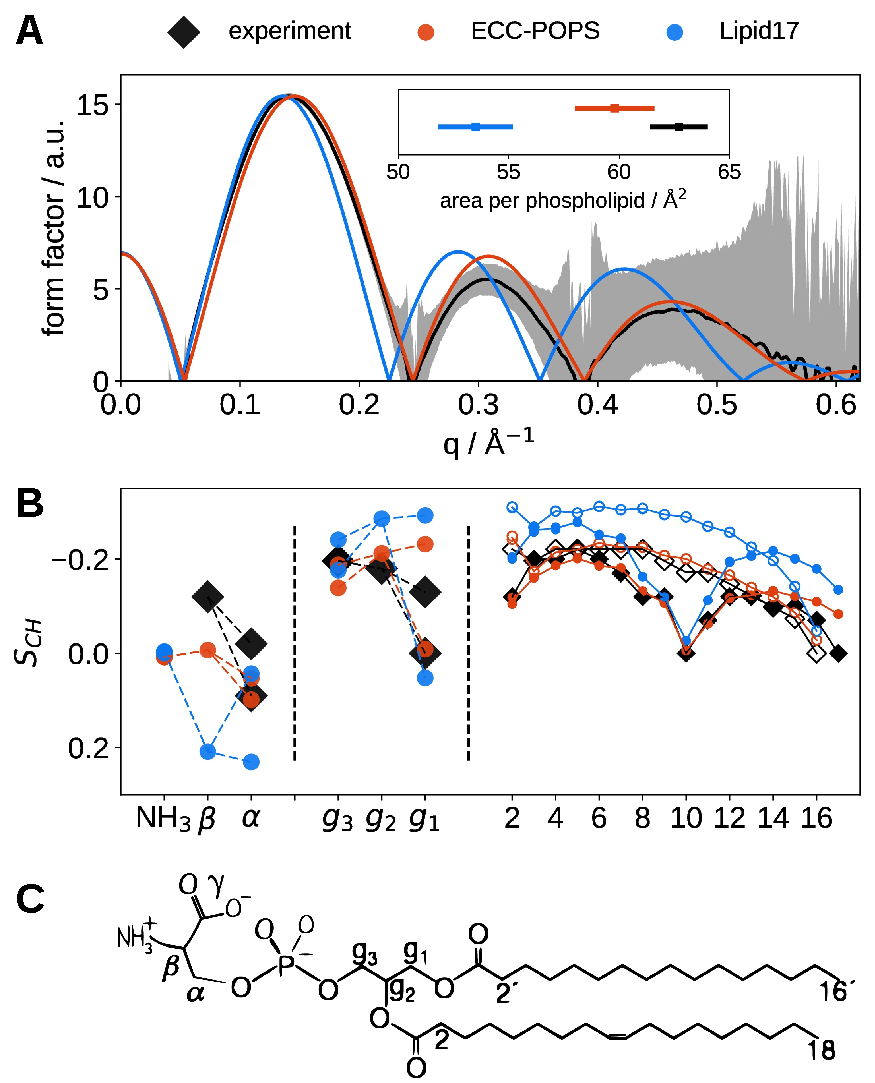
\includegraphics[width=3.33in]{../img/formF_OPs_APLinset_POPSchemfig.pdf} 
\hfill
  \caption{\label{simVSexpNOions_POPS} 
    \textbf{(A)} X-ray scattering form factors and area per phospholipid of a POPS bilayer
    from simulations with Lipid17/Dang \citep{lipid17-future, dang2006} and 
    ECC-POPS/ECC-ions \cite{martinek17, Pluhackova2016} compared with experiments~\citep{kucerka14} at 298~K. 
    \textbf{(B)} Order parameters of POPS headgroup, glycerol backbone and acyl chains  
    from the same simulations 
    compared with experiments at 298~K. \citep{NMRlipidsIV}
    Open/closed symbols are used for palmitoyl/oleoyl chains of POPS. 
    \textbf{(C)} Chemical structure of POPS and labeling of carbon segments. 
  }  
\end{figure} 


The Lipid17/Dang simulation gives 
discrepancies with the experimental X-ray form factor,
larger acyl chain order parameters,
and smaller area per molecule than the experimental values (Fig.~\ref{simVSexpNOions_POPS}),
indicating that this simulation predicts a too compact POPS lipid bilayer. 
The ECC-POPS simulation gives better agreement with experiments for the X-ray scattering form factors and 
acyl chain order parameters (Fig.~\ref{simVSexpNOions_POPS}),
indicating that the bilayer dimensions and acyl chain
conformations are well described by the force field. The area per lipid from ECC-POPS simulation is slightly
smaller than the value reported from SDP model \cite{kucerka14} (Fig.~\ref{simVSexpNOions_POPS}), but the values
agree within their error estimates. The larger area in ECC-POPS compared to Lipid17/Dang simulation can be
explained by increased headgroup repulsion due to lower counterion binding affinity (Fig. \ref{fig:POPS-counterions-dens}).
This explains also the larger area per molecule (57~\AA$^2$) reported for Lipid17 POPS simulations
with {\AA}qvist ion parameters~\cite{NMRlipidsIV}.
However, the Dang ion parameters are used here to analyze the effect of ECC to the properties of a POPS lipid bilayer because
{\AA}qvist ion parameters produce known artifacts, like artificial aggregation of ions at larger salt concentrations \cite{kohagen16, chen07, NMRlipidsIV}.

\begin{figure}[tbp!] 
  \centering 
  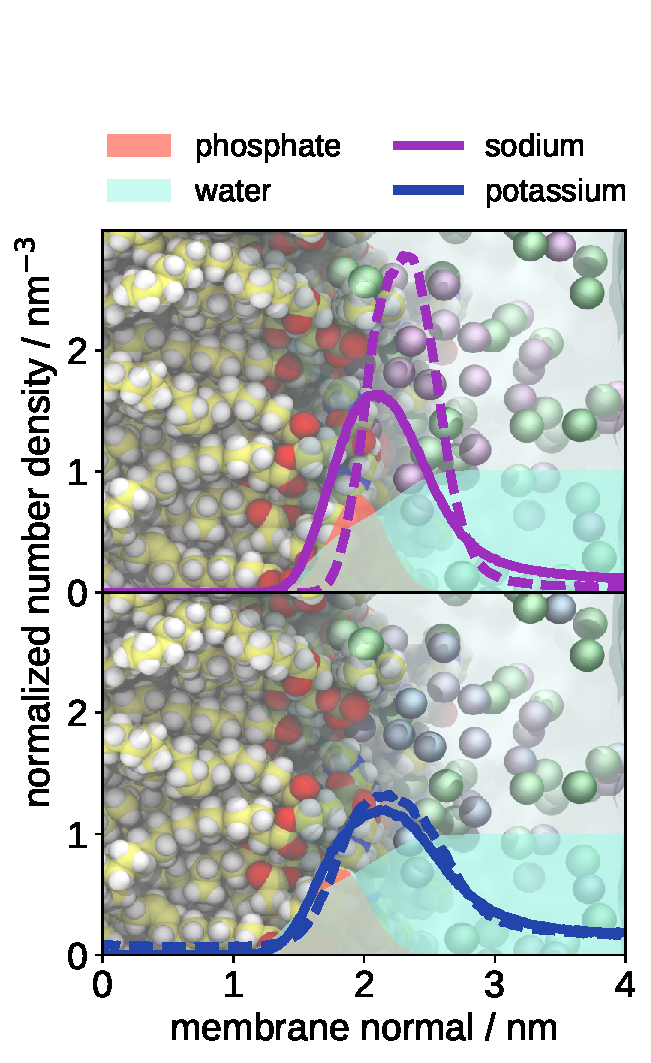
\includegraphics[width=3.33in]{../img/ecc_pops/density_profiles_na-k-counterions_wat_phos_compar_purePOPS_ecclipids-lipid17.pdf}
  \caption{\label{fig:POPS-counterions-dens}
    Number density profiles of \ce{K^{+}} and \ce{Na^{+}} counterions along the membrane normal axis
    in ECC-lipids (solid lines) and Lipid17/Dang (dashed lines) simulations of pure POPS bilayers.  
    The density profiles of phosphate groups and water are divided by 4 and 100, respectively.  
  }
\end{figure}


Despite the success in simulating bilayer dimensions and acyl chain conformations,
lipid force fields have typically problems in capturing the correct glycerol backbone and
headgroup order parameters and conformations \cite{botan15,ollila16,NMRlipidsIV}.
This is the case also for Lipid17 POPS simulations, where the headgroup and glycerol backbone
order parameters are quite far from experimental values with Dang (Fig.~\ref{simVSexpNOions_POPS}),
{\AA}qvist and Joung-Cheatham ion parameters~\cite{NMRlipidsIV}. The values from ECC-POPS simulation are closer,
but not in full agreement with experiments (Fig.~\ref{simVSexpNOions_POPS}).

In conclusion, the stuctural quality of ECC-POPS is similar to the other currently available
lipid force fields \cite{botan15, catte16, Pluhackova2016,NMRlipidsIV},
giving good agreement with experiments for acyl chain conformations and bilayer dimensions,
while there is a room for improvement in the glycerol backbone and headgroup region
conformations.
 
\subsection{Binding of counterions to POPS and POPC and interactions between their headgroups}
Binding affinity of monovalent ions to lipid bilayers depends strongly on
force field parameters in simulations \cite{catte16,NMRlipidsIV}.
The cation binding affinities to lipid bilayers in simulations have been previously evaluated
against experiments using the order parameters of $\alpha$ and $\beta$ carbons in the
phosphatidylcholine (PC) lipid headgroup (see Fig.~\ref{fig:delta_ordPar_monoval_PCPS} for the labeling) \cite{catte16,melcr18,NMRlipidsIV}.
According to the ''electrometer concept'' \citep{seelig87}, these order parameters
decrease proportionally to the amount of bound positive charge because the headgroup dipole tilts more
parallel to the mebrane normal.
Although the response of PS lipid headgroup order parameters to the bound charge is also systematic,
it is less well undestood and the addition of cations may cause phase transitions in negatively charged
bilayers \cite{feigenson86,mattai89,roux91,roux90}.
Therefore, the cation binding affinity to bilayers with PS lipids has been evaluated by measuring the decrease
of PC headgroup order parameters from POPC:POPS (5:1) mixtures upon addition of salt concentration,
which correlate with the amount of bound cations to lipid bilayer according to the
electrometer concept~\cite{akutsu81,altenbach84,seelig87,roux90,catte16,NMRlipidsIV}.
Because the evaluation of monovalent ion binding affinity to bilayers with
PS lipids is complicated by the lack of ion-free state (counterions are always present with negatively charged lipids),
we evaluate the counterion binding affinity to POPC:POPS mixtures also by monitoring
the response of POPC headgroup order parameters to the increasing molar fraction of PS lipids~\cite{NMRlipidsIV} 
(Fig.~\ref{fig:delta_ordPar_NaCl_PC-PS_mix_PC}).

\begin{figure}[tbp!] 
  \centering 
  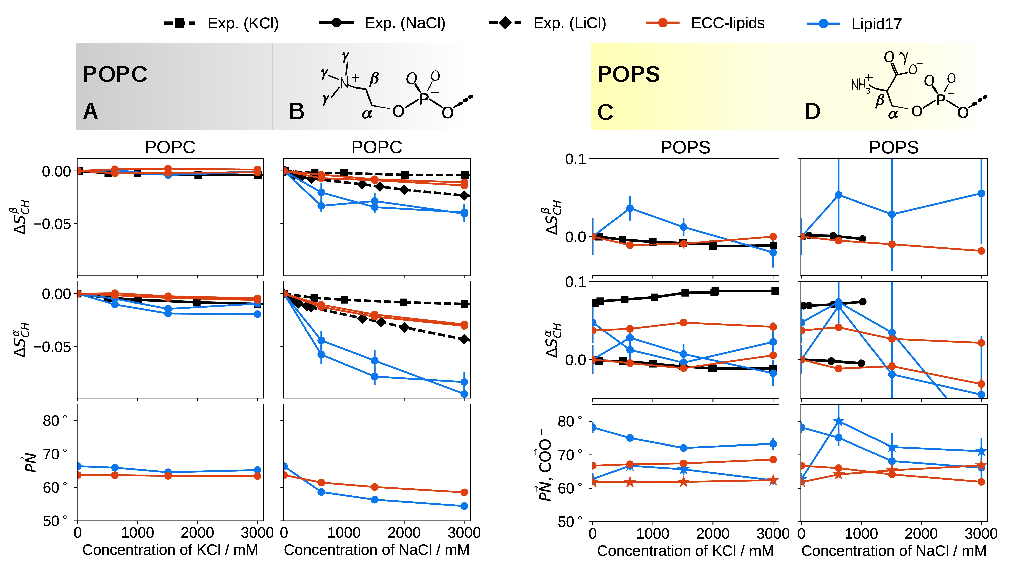
\includegraphics[width=\figwidthfull]{../img/deltaOP_nacl_kcl_PC-PS.pdf} 
  \caption{\label{fig:delta_ordPar_monoval_PCPS}
    Changes of the headgroup order parameters, and the angles of P--N and ${\rm{C}}_\beta-{\rm{C}}_\gamma$ (stars) vectors
    with respect to the membrane normal of POPC (A, B) and POPS (C, D) in a POPC:POPS (5:1) bilayer 
    as a function of \ce{KCl} and \ce{NaCl} concentration from ECC-lipids and Lipid17/Dang simulations 
    compared with experimental values from Ref. \citenum{roux90} (signs from Refs.~\citenum{ferreira16} and~\citenum{NMRlipidsIV}) at 298 K.
    Because experimental data with \ce{NaCl} is not available for POPC, the data for KCl and \ce{LiCl} (B, dashed lines)
    are shown as lower and upper bounds, respectively, for the response to \ce{NaCl}. 
    The y-axis for the $\alpha$-carbon results of POPS (C and D, middle) is shifted
    with the same value for both order parameters such that the lower order
    parameter value from pure POPS is at zero to correctly illustrate the significant forking.
    Error bars are not visible for ECC-lipids simulations because they are smaller than the point size.
    Inset in A shows the labeling of carbon segments in a POPC headgroup.
    For the ion density profiles, see Fig. \ref{fig:nacl-dens_PCPS} in supplementary information.
  }
\end{figure} 


In experiments, the addition of K$^+$ ions led to a very modest decrease of POPC headgroup order parameters in POPC:POPS (5:1) mixture,
while the decrease was more pronounced with Li$^+$ ions and was strongest with divalent Mg$^{2+}$ and Ca$^{2+}$ ions~\cite{roux90},
suggesting that the binding affinity increases in order K$^{+}$ $<$ Li$^{+}$  $<$ Mg$^{2+}$  $<$ Ca$^{2+}$.
The small changes of POPC headgroup order parameters with increasing amount of KCl are close to experiments
in both force fields (Fig.~\ref{fig:delta_ordPar_monoval_PCPS} A).
The slightly overestimated change of the $\alpha$-carbon
order parameter in the Lipid17/Dang simulations may be due to the
deeper penetration of \ce{K+} into the bilayer (Fig.~\ref{fig:delta_ordPar_NaCl_PC-PS_mix_PC} A).
Experimental data with the additional amount of \ce{Na+} in POPC:POPS (5:1) mixture is not available,
but \ce{Li+} and \ce{K+} results give the lower and the upper bounds, respectively, to the sodium binding
affinity (Fig.~\ref{fig:delta_ordPar_monoval_PCPS} B). In ECC-lipids simulations,
the response of POPC headgroup order parameters to the additional sodium is close to the
experimental results for lithium, while in Lipid17/Dang simulations the response is larger.
Overall, the results suggest that the \ce{Na+} binding affinity is
clearly overestimated in Lipid17/Dang simulations and slightly overestimated in ECC-lipids simulations,
while the binding affinity of potassium is better described by both force fields.
This conclusion is also supported by the POPC headgroup responses to the
increasing amount of POPS in different simulations (Fig~\ref{fig:delta_ordPar_NaCl_PC-PS_mix_PC}).
In experiments, the headgroup order parameters of PC lipids increase upon addition of
negatively charged PS lipids, as predicted by the electrometer concept~\cite{seelig87,scherer87}.
This is the case also in simulations with the exception of
Lipid17/Dang with \ce{Na+} counterions, where the stronger counterion binding affinity
cancels the influence of negatively charged lipids and the increase in PC headgroup
order parameters is not observed.

\begin{figure*}[!tbp] 
  \centering 
  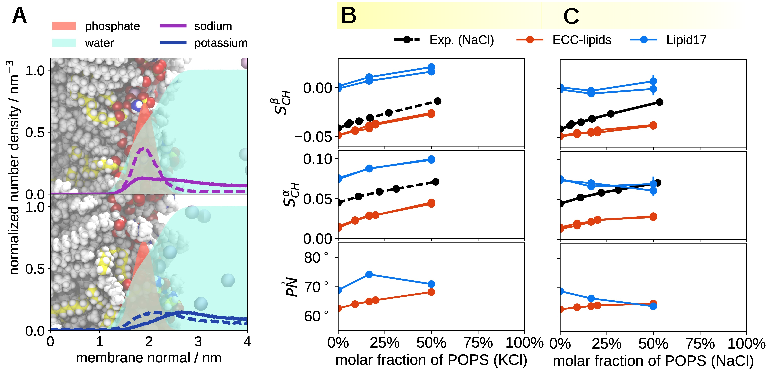
\includegraphics[width=\figwidthfull]{../img/deltaOP_mix_PC-PS.pdf} 
  \caption{\label{fig:delta_ordPar_NaCl_PC-PS_mix_PC} 
    \textbf{(A)} Number density profiles of \ce{K^{+}} and \ce{Na^{+}} counterions along the membrane normal axis
    in ECC-lipids (solid lines) and Lipid17/Dang (dashed lines) simulations of POPC:POPS (5:1) bilayers.  
    The density profiles of phosphate groups and water are divided by 4 and 100, respectively.  
    \textbf{(B, C)} The POPC headgroup order parameters and the P--N vector angle
    with respect to the membrane normal as a function of POPS content in a bilayer
    from ECC-lipids and Lipid17/Dang simulations with \ce{K^+} (B) and \ce{Na^+} (C) counterions.
    Experimental order parameter values with \ce{Na^+} are from Ref. \citenum{scherer87}
    and the signs from Ref.~\citenum{ferreira16}. Because experimental values with \ce{K^+} are
    not available, the data with \ce{Na^+} is shown with dashed lines in (B).
    Error bars are not visible for most of the simulation points because they are smaller than the point size.
    Chemical structure and labelling of carbon segments of POPC is shown in Fig.~\ref{fig:delta_ordPar_monoval_PCPS}. 
  }
\end{figure*} 

The behaviour of POPS headgroup can be further characterized by monitoring its order parameters in different
lipid mixtures and ionic conditions (Figs.~\ref{fig:delta_ordPar_monoval_PCPS} and \ref{fig:delta_ordPar_NaCl_PC-PS_mix_PS})~\cite{NMRlipidsIV,roux90}.
In experiments, the headgroup order parameters of POPS are almost unchanged upon increasing the POPC content or monovalent ion concentration, 
while in Lipid17/Dang simulations the changes of POPS headgroup order parameters with increasing amount of
both POPC or monovalent salts (\ce{KCl} and \ce{NaCl}) are overestimated 
(Figs.~\ref{fig:delta_ordPar_monoval_PCPS} and \ref{fig:delta_ordPar_NaCl_PC-PS_mix_PS}).
Similar results also for other force fields are reported elsewhere~\cite{NMRlipidsIV}.
In ECC-lipids simulations, the response of POPS headgroup order parameters to both POPC and monovalent salt concentration (\ce{KCl} and \ce{NaCl})
are more modest and closer to experiments. 
The changes in order parameters can be related to the orientations of the P--N and C$_{\beta}$--C$_{\gamma}$
vectors in POPC and POPS, which change much less and more systematically in ECC-lipids
than in Lipid17/Dang simulations 
(Figs.~\ref{fig:delta_ordPar_monoval_PCPS} and \ref{fig:delta_ordPar_NaCl_PC-PS_mix_PS}).

We quantify the influence of negatively charged POPS on the counterion binding affinity
by comparing the relative surface excesses with respect to water, $\Gamma ^{w} _{\rm ion}$,
between POPC:POPS (5:1) mixture and pure POPC in ECC-lipids simulations with the most realistic
cation binding affinities~\cite{melcr18}.
The value of $\Gamma ^{w} _{\rm Na}=-0.11 \pm 0.01 \mathrm{nm}^{-2}$ for 1~M sodium in pure ECC-POPC
simulation was reported in the previous work \cite{melcr18}.
The presence of $\sim$17\% POPS in a POPC bilayer increases the
value to $\Gamma ^{w} _{\rm Na}=0.092 \pm 0.005 \mathrm{nm}^{-2}$ 
for 0.621 M sodium, while value for potassium remains negative,
$\Gamma ^{w} _{\rm K}=-0.123 \pm 0.005 \mathrm{nm}^{-2}$ in POPC:POPS (5:1) mixture (Fig.~\ref{fig:nacl-dens_PCPS}).
The increase in sodium binding affinity upon addition of anionic POPS is not expected to depend on
the slightly overestimated \ce{Na+} binding in ECC-lipid simulations, because the
inaccuracy is similar for pure POPC (Fig~3 in Ref.~\citenum{melcr18}) and POPC:POPS (5:1) mixture (Fig. \ref{fig:delta_ordPar_monoval_PCPS}).


\subsection{Molecular interaction and binding affinity of \ce{Ca^{2+}} cations to mixed POPC:POPS (5:1) membrane} 
\label{section:lip-ion_ca}
Our recent work demonstrates that the POPC headgroup order parameters measured
from POPC:POPS (5:1) mixture as a function of CaCl$_2$ concentration 
can be used to evaluate the calcium binding affinity to lipid bilayers containing PS lipids \cite{roux90,NMRlipidsIV}.
The decrease of the PC headgroup order parameters in this mixture upon addition of \ce{CaCl2} 
were overestimated by the Lipid17/Dang simulations (Fig.~\ref{fig:delta_ordPar_CaCl_PCPS})
and all other tested force fields except CHARMM36 with the recently introduced NBfix parameters for calcium \cite{kim16,han2018graph},
which underestimated the headgroup order parameter response.
In ECC-lipids simulations, the headgroup responses are in better agreement with experiments,
indicating that the lower binding affinity than in Lipid17/Dang simulations is more realistic (Fig.~\ref{fig:cacl-dens_PCPS}).
Therefore, we use ECC-lipids simulations to quantify the influence of negative charged POPS on
calcium binding affinity to lipid bilayers.
The relative surface excess of calcium with respect to water 
$\Gamma^{w}_{Ca} = 0.09\mathrm{nm^{-2}}$
for pure POPC bilayer with 467~mM CaCl$_2$ \cite{ECC-POPC_nacl_cacl2_files}
is increased to
$\Gamma^{w}_{Ca} = 0.24\mathrm{nm^{-2}}$
for the POPC:POPS (5:1) bilayer with 409 mM CaCl$_2$.
With these concentrations, the total amount of lipids per bound \ce{Ca^{2+}} is
$\sim 5.4$ in the pure POPC system and $\sim 4.8$ in the POPC:POPS (5:1) mixture.
Interestingly, the calcium residence times are 3-4 times longer in POPC:POPS (5:1) mixture (Fig.~\ref{fig:hist_residence_times}) than in pure POPC \cite{melcr18}.
Besides lower binding affinity, ECC-lipids simulations yield smaller error bars for order parameters and shorter residence times (Fig.~\ref{fig:hist_residence_times}) 
than those typically observed in simulations with other force fields \cite{javanainen17,melcr18,NMRlipidsIV},
suggesting that the ECC accelerates the equilibration of ions at lipid bilayer interface.
Therefore, our 1 $\mu$s simulations are sufficiently long for the ECC-lipids simulations, because
90\% of the calcium residence times are shorter than $60\,\mathrm{ns}$ for pure POPC bilayer
and shorter than $200\,\mathrm{ns}$ for POPC:POPS (5:1) mixture, while the
longest observed residence times are $141\,\mathrm{ns}$ and $485\,\mathrm{ns}$, respectively (Fig.~\ref{fig:hist_residence_times}).



\begin{figure}[tbp!] 
  \centering 
  \begin{tabular}{ c }
  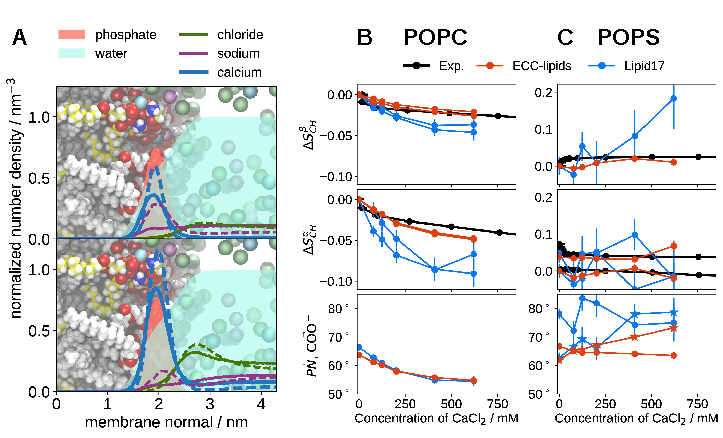
\includegraphics[width=\figwidthfull]{../img/deltaOP_cacl_PC-PS.pdf} 
  \end{tabular}
  \caption{
    \label{fig:cacl-dens_PCPS} 
    \label{fig:delta_ordPar_CaCl_PCPS} 
    \textbf{(A)}
    Number density profiles of \ce{Ca^{2+}} and \ce{Cl^-} ions and \ce{Na^{+}} counterions 
    along the normal of POPC:POPS (5:1) bilayer with 80~mM (A, top) and 200~mM (A, bottom)
    of \ce{CaCl2} from simulations with ECC-lipids (solid) and Lipid17 (dashed). 
    The~\ce{Ca^{2+}}, phosphate and water densities are divided by 2, 4 and 100, respectively.  
    \textbf{(B, C)}
    Changes of the headgroup order parameters, and the angles of P--N (circles) and C$_\beta$--C$_\gamma$ (stars) vectors 
    with respect to the membrane normal of POPC (B) and POPS (C) in a POPC:POPS (5:1) bilayer 
    as a function of \ce{CaCl$_2$} from ECC-lipids and Lipid17/Dang simulations 
    compared with experimental values from Ref. \citenum{roux90} (signs from Refs. \citenum{ferreira16} and \citenum{NMRlipidsIV}) at 298 K.
    The y-axis for the $\alpha$-carbon results of POPS (C, right) is shifted
    with the same value for both order parameters such that the lower order
    parameter value from pure POPS is at zero to correctly illustrate the significant forking.
    Error bars are not visible for ECC-lipids simulations because they are smaller than the point size.
  }
\end{figure}

\begin{figure}[tbp!] 
  \centering 
  \begin{tabular}{ c }
  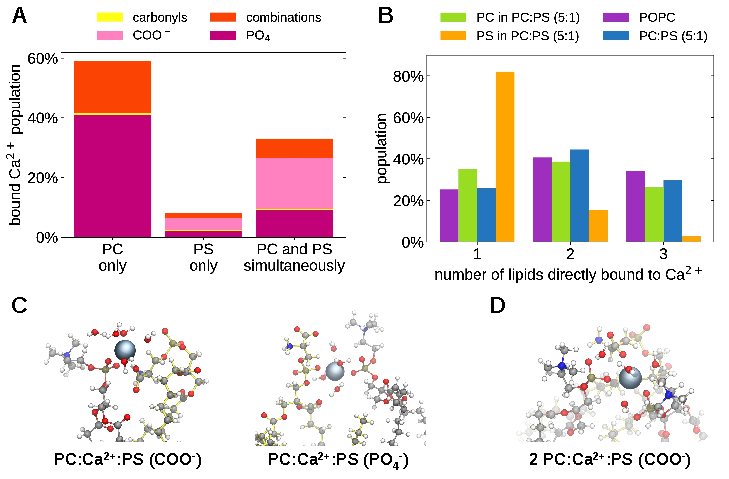
\includegraphics[width=\figwidthfull]{../img/populations_stoichiometry_structures.pdf} 
  \end{tabular}
  \caption{ \label{fig:cacl_complexes} 
    \textbf{(A)} Percentages of the bound Ca$^{2+}$ 
    in exclusive contact with the given oxygen moiety
    when bound to PC only, PS only or simultaneously to both
    calculated from ECC-lipids simulation of POPC:POPS (5:1) bilayer with 409 mM CaCl$_2$. 
	In the case of simultaneous binding to both PC and PS,
	the percentages refer to the moieties in PS.
        For numerical values, see table~\ref{tab:binding}.
    \textbf{(B)} Relative probabilities of \ce{Ca^{2+}} ions to coordinate with the given number of lipids
    in a pure POPC bilayer with 350~mM~CaCl$_2$ and in POPC:POPS (5:1) mixture with 400~mM~CaCl$_2$.  
    Analysis was done for both systems by considering all lipids (blue and violet) and
    for POPC:POPS (5:1) mixture also by considering only POPC and POPS lipids separately (green and orange). 
    Clusters of four or more lipids were not observed in either membrane.
    The threshold for counting coordinated lipids in a complex with \ce{Ca^{2+}} was set to $0.3\,\mathrm{nm}$, 
    for the distance between the cation and the oxygen atoms of the lipids. 
    \textbf{(C and D)} Representative example configurations of \ce{Ca^{2+}} coordinated complexes 
    of one POPS with one POPC (C) or two POPC lipids (D). 
    Extra configurations are given in Fig.~\ref{fig:strcutures_SI} in the SI. 
    Previously published simulation data \cite{melcr18} for pure POPC bilayers were taken directly from Ref.~\citenum{ECC-POPC_nacl_cacl2_files}. 
  }
\end{figure} 

Interactions between Ca$^{2+}$ ions and PS lipids can be further characterized by monitoring
the POPS headgroup order parameters from POPC:POPS (5:1) mixture with increasing  CaCl$_2$ concentration~\cite{roux90}.
In experiments, the headgroup order parameters of POPS exhibit a strong dependence
on low CaCl$_2$ concentrations with a rapid saturation below 100~mM  (Fig.~\ref{fig:delta_ordPar_CaCl_PCPS}) \cite{roux90}.
These changes are overestimated in simulations with Lipid17/Dang (Fig.~\ref{fig:delta_ordPar_CaCl_PCPS})
and other tested force fields in our recent work \cite{NMRlipidsIV}, 
including CHARMM36 with the NBfix corrections for calcium
which underestimated the binding affinity.
In ECC-lipids simulations, the changes of the PS headgroup order parameters are not overestimated,
but the strong dependence on low concentrations of CaCl$_2$ is not fully reproduced (Fig.~\ref{fig:delta_ordPar_CaCl_PCPS}).
In addition to possibly suboptimal interactions between calcium ions and PS headgroup, the potential sources of this
discrepancy include the above observed slight overestimation of \ce{Na^+} counterions and
imperfect structures of the lipid headgroup (Fig.~\ref{simVSexpNOions_POPS}).

Recent analyzes of interaction sites between calcium and PS lipids combining
MD simulations with various experimental techniques have been 
controversial because the results strongly depend on force fields parameters \cite{melcrova16,valentine18,hallock18}.
Here, we analyze the calcium binding details from ECC-lipids simulation of POPC:POPS (5:1) mixture with 409 mM CaCl$_2$,
because it surpasses the quality of other force fields in direct comparison with experimental order parameter data.
In the ECC-lipid simulation, calcium ions binds approximately twice more likely 
to the carboxylate than to the phosphate moiety of POPS headgroup,
while binding to acyl chain carbonyls is almost negligible (Fig.~\ref{fig:cacl_complexes} and Table~\ref{tab:binding}).
The result is consistent with CHARMM36 simulations without the NBfix correction \cite{hallock18},
but CHARMM36 simulations with the NBfix correction \cite{kim16} predict almost exclusive binding to carboxylate group \cite{valentine18}
and Berger simulations show signifincant binding affinity also to acyl chain carbonyls \cite{melcrova16}.
On the other hand, calcium ions bind too strongly on bilayers simulated using CHARMM36 without the NBfix correction
or Berger models, and too weakly on CHARMM36 bilayers with the NBfix correction \cite{catte16,NMRlipidsIV}.
Furthermore, in CHARMM36 simulations without the NBfix,
calcium ions coordinate with even four distinct PS lipids \cite{hallock18}, while coordination with more than two PS lipids
is very rare in our ECC-lipids simulations (Fig.~\ref{fig:cacl_complexes}).

The improved accuracy in ECC-lipids simulations motivates also the more detailed analysis of
POPS headgroup response to the bound calcium ions, which is potentially important in calcium regulated
lipid-protein interactions \cite{leventis10}.
Upon addition of 620~mM CaCl$_2$ to POPC:POPS (5:1) mixture,
the average orientation of P--N vectors in both POPC and POPS headgroups tilts more perpendicular to the membrane surface
by 11$^\circ$ and  3$^\circ$, respectively, in ECC-lipids simulations (Fig.~\ref{fig:delta_ordPar_CaCl_PCPS}),
suggesting that the PS headgroup orientation is less sensitive to the bound calcium than PC.
On the other hand, the average orientation of the C$_{\beta}$--C$_{\gamma}$ vector in PS headgroup
tilts to the opposite direction by $11^\circ$ in the same system, probably
due to the attraction between \ce{COO^-} groups and cations adsorbed at the phosphate region.



\section{Conclusions} 
We have applied ECC to implicitly include electronic polarization to the Amber Lipid17 force field
parameters of negatively charged POPS lipid.
Because PS headgroup bears a unit negative charge, we apply the scaling factor of 0.75,
derived for monovalent ions~\cite{leontyev09}, to the partial charges
in the headgroup, glycerol backbone and carbonyl regions of POPS.
Following our previous work for zwitterionic POPC lipids, the 
Lennard-Jones $\sigma$ parameters of the same POPS segments were
scaled by a factor of 0.89 to optimize the hydration properties of the bilayer~\cite{melcr18}.
Similarly to other state of the art lipid models, the created ECC-POPS parameters give
lipid bilayer dimensions and acyl chain structures in agreement with experiments,
but leaves room for improvement for the headgroup structure when validated against
NMR and scattering experiments~\cite{botan15,ollila16}.
Nevertheless, ECC-lipid parameters describe cation (Na$^+$ and Ca$^{2+}$) binding affinities
and their interactions with PS headgroups better than other available lipid force fields,
when validated using the headgroup order parameters and ``electrometer concept''~\cite{NMRlipidsIV}.
There is, however, room for improvement in capturing the sensitive headgroup responses to the
small concentrations of CaCl$_2$.

In our ECC-lipids simulation, Ca$^{2+}$ ions bind twice more likely to carboxylate groups
of PS headgroups than to phosphate groups, while binding to carbonyls is almost negligible.
Binding of Ca$^{2+}$ ions to more than two POPS lipids simultaneously is very rare in \mbox{ECC-lipids} simulations.
Because \mbox{ECC-lipids} parameters give the best results in direct comparison with NMR order parameters, 
we believe that our results help in resolving controversial interpretations of more indirect experiments
using different force fields~\cite{melcrova16,valentine18,hallock18}.
Furthermore, our results pave the way for more realistic MD simulations of anionic biological membranes,
and demonstrate the usefulness of ECC also for charged lipids.

The general philosophy behind our approach is to build upon existing non-polarizable force fields making the minimum of necessary changes by scaling only groups bearing a sizeable (partial) charge, followed by slight readjustments of van der Waals radii and possibly also other parameters such as those concerning dihedral angle terms.
The present work thus represents another piece in the mosaic that leads to development of an accurate empirical force field for biomolecular simulations involving aqueous salt solutions, proteins, peptides, lipid membranes, and/or nucleic acids, which include electronic polarization effects in a mean field way via charge scaling without extra computational costs compared to standard non-polarizable simulations. 
We believe that ECC corrected lipid force fields will be useful in modelling complex biomembranes when 
explicitly polarizable force fields for lipids \cite{li17,chu18} are not necessary.

% If you have acknowledgments, this puts in the proper section head. 
\begin{acknowledgement} 
% Put your acknowledgments here. 
P.J. acknowledges support from the Czech Science Foundation via an EXPRO grant no. 19-26854X. 
Computational resources were supplied by the Ministry of Education, Youth and Sports 
of the Czech Republic under the Projects CESNET (Project No. LM2015042) and CERIT-Scientific 
Cloud (Project No. LM2015085) provided within the program Projects of Large Research, 
Development and Innovations Infrastructures. 
O.H.S.O. acknowledges financial support from Academy of Finland (315596),
Integrated Structural Biology Research Infrastructure of
Helsinki Institute of Life Science (Instruct-HiLIFE), and
CSC-IT center for science for computational resources.
\end{acknowledgement} 
 
\begin{suppinfo} 
 
%A listing of the contents of each file supplied as Supporting Information 
%should be included. For instructions on what should be included in the 
%Supporting Information as well as how to prepare this material for 
%publications, refer to the journal's Instructions for Authors. 
 
The following files are available free of charge. 
\begin{itemize} 
  \item SI.pdf: Additional simulation and experimental details, figures and tables. 
\end{itemize} 
 
\end{suppinfo} 
 
 
\bibliography{refs.bib} 
 
\end{document} 
 

